\documentclass[12pt]{article}
\usepackage{amsmath, amssymb, amsfonts, bm, graphicx, geometry, tabularx, booktabs, float, enumitem, cancel}
\geometry{margin=1in}

\title{}
\date{}
\author{}

% Uppercase Volume with thicker, higher line
\newcommand{\vol}{\mathord{\text{\ooalign{\hidewidth $V$\hidewidth\cr\kern-0.5pt\raisebox{0.8ex}{\rule[0pt]{1em}{0.5pt}}}}}}

% Lowercase Volume with built-in shifts
\newcommand{\svol}{%
  \mathord{\text{\ooalign{%
    \hfil$v$\hfil\cr
    \hfil\rule[0.6ex]{0.8em}{0.5pt}\hfil
  }}}%
}

\begin{document}
\noindent
\underline{Note:} When doing any first law analysis, always define the control volume with a sketch!
\section*{5-28E}
\vspace{-2em}
\begin{center}
    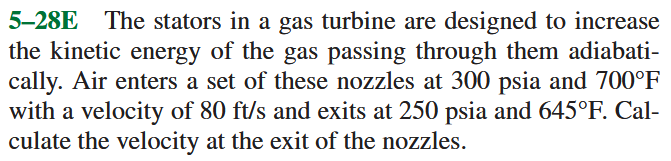
\includegraphics[width=0.7\textwidth]{5-28E.png}
\end{center}
Given:
\begin{itemize}
    \item State 1 (entering nozzle)
    \begin{itemize}
        \item $P_1 = 300$ psia, $T_1 = 700^\circ$F, $v_1 = 80 \,\text{ ft}/\text{s}$
    \end{itemize}
    \item State 2 (exiting nozzle)
    \begin{itemize}
        \item $P_2 = 250$ psia, $T_2 = 645^\circ$F
    \end{itemize}
    \item Adiabatic process (no heat transfer, $\dot{Q}=0$)
\end{itemize}
Find: 
\begin{itemize}
    \item Velocity at state 2, $v_2$
\end{itemize}
Writing the first law of thermodynamics for an open system (nozzle):
\[\frac{dE}{dt} = \dot{Q}-\dot{W} +
\sum \dot{m_i}\left[h_i+\frac{1}{2}v_i^2+g z_i\right]
-\sum \dot{m_e}\left[h_e+\frac{1}{2}v_e^2+g z_e\right]\]
We can simplify the first law eqn for this system as follows:
\begin{itemize}
\item No work is done by the system ($\dot{W}=0$), it only increases the velocity of the gas
\item No heat transfer ($\dot{Q}=0$)
\item Steady state ($\frac{dE}{dt}=0$), because there is no accumulation of energy in the system over time
\item Neglect potential energy changes ($g z_i \approx g z_e$)
\end{itemize}
Thus, the first law simplifies to:
\[\dot{m}_1 \left(h_1 +\frac{1}{2}v_1^2\right) = \dot{m}_2 \left(h_2 +\frac{1}{2}v_2^2\right)\]
Applying the conservation of mass:
\[\frac{dm}{dt} = \sum \dot{m}_i - \sum \dot{m}_e\]
\[\implies \dot{m}_1 = \dot{m}_2\]
Therefore:
\[h_1 +\frac{1}{2}v_1^2 = h_2 +\frac{1}{2}v_2^2\]
Now there are two ways to determine the specific enthalpies $h_1$ and $h_2$:\\\\
\textbf{Method 1: Using Property Tables}\\
Using table A-17E (ideal gas properties for air), we can find the specific enthalpies at the given states:
\begin{itemize}
    \item At state 1 ($P_1=300$ psia, $T_1=700^\circ\text{F} = 1159.67\,\text{R}$):
    \begin{itemize}
        \item $h_1 = 281.14$ Btu/lbm
    \end{itemize}
    \item At state 2 ($P_2=250$ psia, $T_2=645^\circ\text{F} = 1104.67\,\text{R}$):
    \begin{itemize}
        \item Using linear interpolation between the values at $T=1080\,\text{R}$ and $T=1120\,\text{R}$:
        \[h-h_{1080} = \frac{h_{1120}-h_{1080}}{T_{1120}-T_{1080}}(T-T_{1080})\]
        \[h_2 = 267.17 \text{ Btu/lbm}\]
    \end{itemize}
\end{itemize}
Substituting the values into the first law equation:
\[v_2 = \sqrt{2(h_1 - h_2) + v_1^2}\]
\[v_2 = \sqrt{2\left[281.14-267.17\,\frac{\cancel{\text{Btu}}}{\cancel{\text{lbm}}}\cdot\frac{778.169\,\text{ft}\cdot\cancel{\text{lbf}}}{1\,\cancel{\text{Btu}}}\cdot\frac{32.174\,\frac{\cancel{\text{lbm}}\cdot\text{ft}}{\text{s}^2}}{1\,\cancel{\text{lbf}}}\right]+\left[80\,\frac{\text{ft}}{\text{s}}\right]^2} = \boxed{840.195\,\frac{\text{ft}}{\text{s}}}\]
\textbf{Method 2: Using Ideal Gas Relations}\\
Assuming that air behaves as an ideal gas and that the specific heats are constant (we can usually assume this unless stated otherwise), we can use the following relation:
\[(h_2 - h_1) = c_p (T_2 - T_1)\]
For air at 700$^\circ$F, $c_p = 0.254 \text{ Btu/lbm}\cdot\text{R}$, so:
\[h_1 - h_2 = -c_p (T_2 - T_1) = -\left[0.254 \,\frac{\text{Btu}}{\text{lbm}\cdot\text{R}}\right][1104.67 - 1159.67 \,\text{R}]=13.97\,\frac{\text{Btu}}{\text{lbm}}\]
Substituting into the first law equation:
\[v_2 = \sqrt{2\left[13.97\,\frac{\cancel{\text{Btu}}}{\cancel{\text{lbm}}}\cdot\frac{778.169\,\text{ft}\cdot\cancel{\text{lbf}}}{1\,\cancel{\text{Btu}}}\cdot\frac{32.174\,\frac{\cancel{\text{lbm}}\cdot\text{ft}}{\text{s}^2}}{1\,\cancel{\text{lbf}}}\right]+\left[80\,\frac{\text{ft}}{\text{s}}\right]^2} = 840.195\,\frac{\text{ft}}{\text{s}}\]
Note that the specific heat values are dependent on temperature, so if we used the specific heat at the wrong temperature, we would see a larger error.

\section*{5-47}
\vspace{-2em}
\begin{center}
    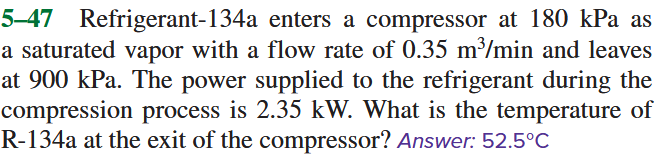
\includegraphics[width=0.7\textwidth]{5-47.png}
\end{center}
Given:
\begin{itemize}
    \item State 1 (compressor inlet)
    \begin{itemize}
        \item Saturated vapor at $P_1 = 180$ kPa, $\dot{v}_1 = 0.35 \text{ m}^3/\text{min}$
        \item Because it is a saturated vapor, we can find its properties from the property tables:
        \begin{itemize}
            \item $T_1 = T_\text{sat} = -12.73^\circ\text{C}$
            \item $h_1 = h_g = 242.90$ kJ/kg
            \item $\svol_1 = \svol_g = 0.11049 \text{ m}^3/\text{kg}$
        \end{itemize}
    \end{itemize}
    \item State 2 (compressor outlet)
    \begin{itemize}
        \item $P_2 = 900$ kPa
    \end{itemize}
    \item Power supplied to compressor, $\dot{W} = 2.35$ kW
\end{itemize}
Find: 
\begin{itemize}
    \item Temperature at state 2, $T_2$
\end{itemize}
Writing the first law of thermodynamics for an open system (compressor):
\[\frac{dE}{dt} = \dot{Q}-\dot{W} +
\sum \dot{m_i}\left[h_i+\frac{1}{2}v_i^2+g z_i\right]
-\sum \dot{m_e}\left[h_e+\frac{1}{2}v_e^2+g z_e\right]\]
We can simplify the first law eqn for this system as follows:
\begin{itemize}
\item No heat transfer ($\dot{Q}=0$)
\item Steady state ($\frac{dE}{dt}=0$), because there is no accumulation of energy in the system over time
\item Neglect potential energy changes ($g z_i \approx g z_e$)
\item Neglect kinetic energy changes ($\frac{1}{2}v_i^2 \approx \frac{1}{2}v_e^2$), because the compressor primarily ONLY increases the pressure, not the velocity
\end{itemize}
Thus, the first law simplifies to:
\[0 = -\dot{W} + \dot{m}_1h_1 - \dot{m}_2h_2\]
Applying the conservation of mass:
\[\frac{dm}{dt} = \sum \dot{m}_i - \sum \dot{m}_e\quad \implies \dot{m}_1 = \dot{m}_2\]
Therefore:
\[\dot{W} = \dot{m}_1(h_1 - h_2)\]
Solve for the mass flow rate $\dot{m}_1$:
\[\dot{m} = \rho \dot{\vol} = \frac{\dot{\vol}}{\svol}\]
\[\dot{m}_1 = \frac{\left[0.35\,\frac{\text{m}^3}{\text{min}} \cdot \frac{1\,\text{min}}{60\,\text{s}}\right]}{\left[0.11049\,\frac{\text{m}^3}{\text{kg}}\right]} = 0.05279\,\frac{\text{kg}}{\text{s}}\]
Plugging in the values to solve for $h_2$:
\[h_2 = h_1 - \frac{\dot{W}}{\dot{m}_1} = \left[242.90\,\frac{\text{kJ}}{\text{kg}}\right] - \frac{\left[-2.35\,\text{kW}\cdot \frac{1\,\frac{\text{kJ}}{\text{s}}}{1\,\text{kW}}\right]}{\left[0.05279\,\frac{\text{kg}}{\text{s}}\right]}=287.416\,\frac{\text{kJ}}{\text{kg}}\]
\underline{Note:} Energy IN is always negative by our sign convention!\\\\
Based on $h_2$ we can determine the state of the refrigerant at state 2. At $P_2=900$ kPa, $h_g = 269.31$ kJ/kg, therefore the refrigerant is a \textit{superheated vapor}. Based on the superheated vapor tables, we can then find the temperature at state 2 using linear interpolation between the values at ($T=50^\circ\text{C}$, $h= 284.79$ kJ/kg) and ($T=60^\circ\text{C}$, $h= 295.15$ kJ/kg):
\[T - T_{50} = \frac{T_{60} - T_{50}}{h_{60} - h_{50}} (h - h_{50})\]
\[\boxed{T_2 = 52.53^\circ\text{C}}\]
\newpage

\section*{5-57}
\vspace{0em}
\begin{center}
    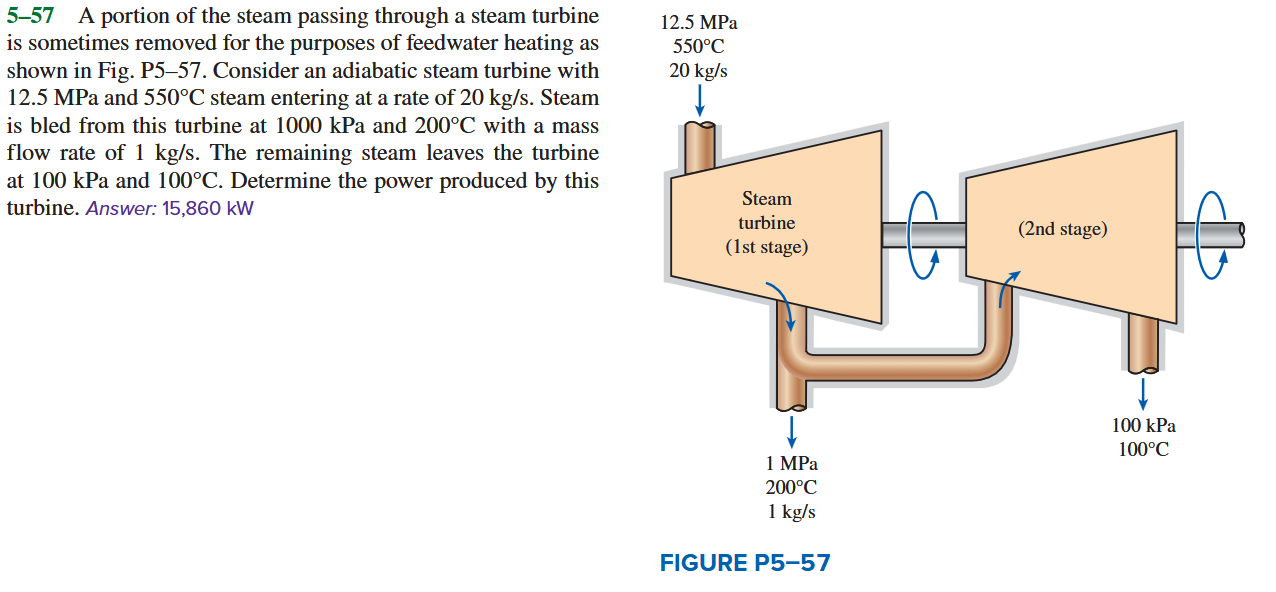
\includegraphics[width=1\textwidth]{5-57.png}
\end{center}
\vspace{-2em}
Given:
\begin{itemize}
    \item State 1 (entering 1st stage)
    \begin{itemize}
        \item $P_1 = 12.5$ MPa, $T_1 = 550^\circ$C, $\dot{m}_1 = 20 \,\text{ kg}/\text{s}$
    \end{itemize}
    \item State 2 (exiting 1st stage)
    \begin{itemize}
        \item $P_2 = 1$ MPa, $T_2 = 200^\circ$C, $\dot{m}_2 = 1 \,\text{ kg}/\text{s}$
    \end{itemize}
    \item State 3 (entering 2nd stage)
    \begin{itemize}
        \item $P_3 = 1$ MPa, $T_3 = 200^\circ$C, $\dot{m}_3 = 20-1 = 19 \,\text{ kg}/\text{s}$
    \end{itemize}
    \item State 4 (exiting 2nd stage)
    \begin{itemize}
        \item $P_4 = 0.1$ MPa, $T_4 = 100^\circ$C, $\dot{m}_4 = \dot{m}_3 = 19 \,\text{ kg}/\text{s}$
    \end{itemize}
    \item Adiabatic process (no heat transfer, $\dot{Q}=0$) with STEAM
\end{itemize}
Find: 
\begin{itemize}
    \item Power produced by the turbine, $\dot{W}$
\end{itemize}
Writing the first law of thermodynamics for an open system (both stages of the turbine):
\[\frac{dE}{dt} = \dot{Q}-\dot{W} +
\sum \dot{m_i}\left[h_i+\frac{1}{2}v_i^2+g z_i\right]
-\sum \dot{m_e}\left[h_e+\frac{1}{2}v_e^2+g z_e\right]\]
Since the turbine's main purpose is to convert the enthalpy of the steam into work, we can simplify the first law equation as follows:
\begin{itemize}
\item No heat transfer ($\dot{Q}=0$)
\item Steady state ($\frac{dE}{dt}=0$), because there is no accumulation of energy in the system over time
\item Neglect potential energy changes ($g z_i \approx g z_e$)
\item Neglect kinetic energy changes ($\frac{1}{2}v_i^2 \approx \frac{1}{2}v_e^2$), because the compressor primarily ONLY increases the pressure, not the velocity
\end{itemize}
Thus, the first law simplifies to:
\[\dot{W} = \left[\dot{m}_1 h_1\right] - \left[\dot{m}_2 h_2 + \dot{m}_4 h_4\right]\]
Using the superheated water tables, we can find the specific enthalpies: $h_1 = 3476.5$ kJ/kg, $h_2 = 2828.3$ kJ/kg, and $h_4 = 2675.8$ kJ/kg.\\\\
Substituting into the first law equation:
\[\dot{W} = \left[20\,\frac{\text{kg}}{\text{s}} \cdot 3476.5\,\frac{\text{kJ}}{\text{kg}}\right] - \left[1\,\frac{\text{kg}}{\text{s}} \cdot 2828.3\,\frac{\text{kJ}}{\text{kg}} + 19\,\frac{\text{kg}}{\text{s}} \cdot 2675.8\,\frac{\text{kJ}}{\text{kg}}\right] = \boxed{15861.5\,\frac{\text{kJ}}{\text{s}}}\]

\section*{5-63}
\vspace{-2em}
\begin{center}
    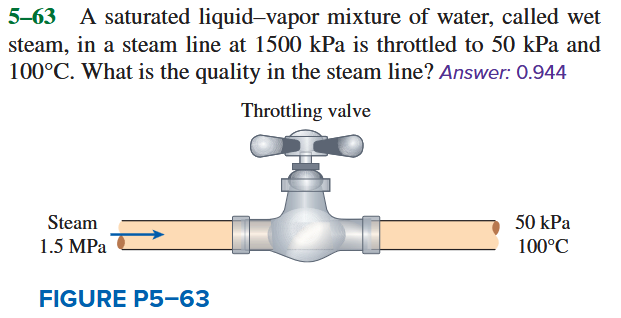
\includegraphics[width=0.6\textwidth]{5-63.png}
\end{center}
Given:
\begin{itemize}
    \item State 1 (entering the valve)
    \begin{itemize}
        \item $P_1 = 1.5$ MPa
        \item It is a saturated liquid-vapor mixture at state 1.
    \end{itemize}
    \item State 2 (exiting the valve)
    \begin{itemize}
        \item $P_2 = 50$ kPa, $T_2 = 100^\circ$C
        \item At $50$ kPa, $T_\text{sat} = 81.34^\circ$C, so the steam is a superheated vapor at state 2. From the superheated water tables, we can find $h_2 = 2682.4$ kJ/kg.
    \end{itemize}
\end{itemize}
Find: 
\begin{itemize}
    \item Quality of the steam at state 1, $x_1$
\end{itemize}
Writing the first law of thermodynamics for an open system:
\[\frac{dE}{dt} = \dot{Q}-\dot{W} +
\sum \dot{m_i}\left[h_i+\frac{1}{2}v_i^2+g z_i\right]
-\sum \dot{m_e}\left[h_e+\frac{1}{2}v_e^2+g z_e\right]\]
A throttling process is similar to a nozzle, except that the main role of a throttling process is to reduce the pressure of the fluid, not to increase its velocity. Therefore, we can simplify the first law equation as follows:
\begin{itemize}
\item No work is done by the system ($\dot{W}=0$), it only reduces the pressure of the fluid
\item No heat transfer ($\dot{Q}=0$)
\item Steady state ($\frac{dE}{dt}=0$), because there is no accumulation of energy in the system over time
\item Neglect potential energy changes ($g z_i \approx g z_e$)
\item Neglect kinetic energy changes ($\frac{1}{2}v_i^2 \approx \frac{1}{2}v_e^2$)
\item By conservation of mass, $\dot{m}_1 = \dot{m}_2$
\end{itemize}
Thus, the first law simplifies to:
\[0 = h_1 - h_2 \quad \implies \quad h_1 = h_2\]
\underline{Note:} In a throttling process, the enthalpy of the fluid remains constant!\\\\
Therefore, using $h_1 = h_2$, we can find the quality of the steam at state 1:
\[x = \frac{h_1 - h_f}{h_{fg}} = \frac{[2682.4\ - 844.55\,\text{kJ}/\text{kg}]}{[1946.4\,\text{kJ}/\text{kg}]} = \boxed{0.944}\]

\section*{5-73}
\vspace{-2em}
\begin{center}
    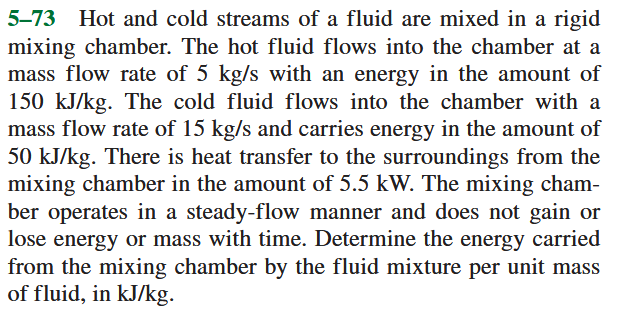
\includegraphics[width=0.6\textwidth]{5-73.png}
\end{center}
\newpage\noindent
Given:
\begin{itemize}
    \item State 1 (hot fluid entering the mixing chamber)
    \begin{itemize}
        \item $\dot{m}_1 = 5$ kg/s, $h_1 = 1500$ kJ/kg
    \end{itemize}
    \item State 2 (cold fluid entering the mixing chamber)
    \begin{itemize}
        \item $\dot{m}_2 = 15$ kg/s, $h_2 = 50$ kJ/kg
    \end{itemize}
    \item State 3 (mixture exiting the mixing chamber)
    \begin{itemize}
        \item $\dot{m}_3 = \dot{m}_1 + \dot{m}_2$
    \end{itemize}
    \item Heat transfer \textit{from the system} to the surroundings, $\dot{Q} = 5.5$ kW
\end{itemize}
Find: 
\begin{itemize}
    \item Specific enthalpy of the mixture at state 3, $h_3$ [kJ/kg]
\end{itemize}
The system operates in a \textbf{steady-flow} manner, this means that there is no accumulation of energy or mass in the system over time. This is why we know there must be a $\dot{m}_3$ exiting the system:
\begin{center}
    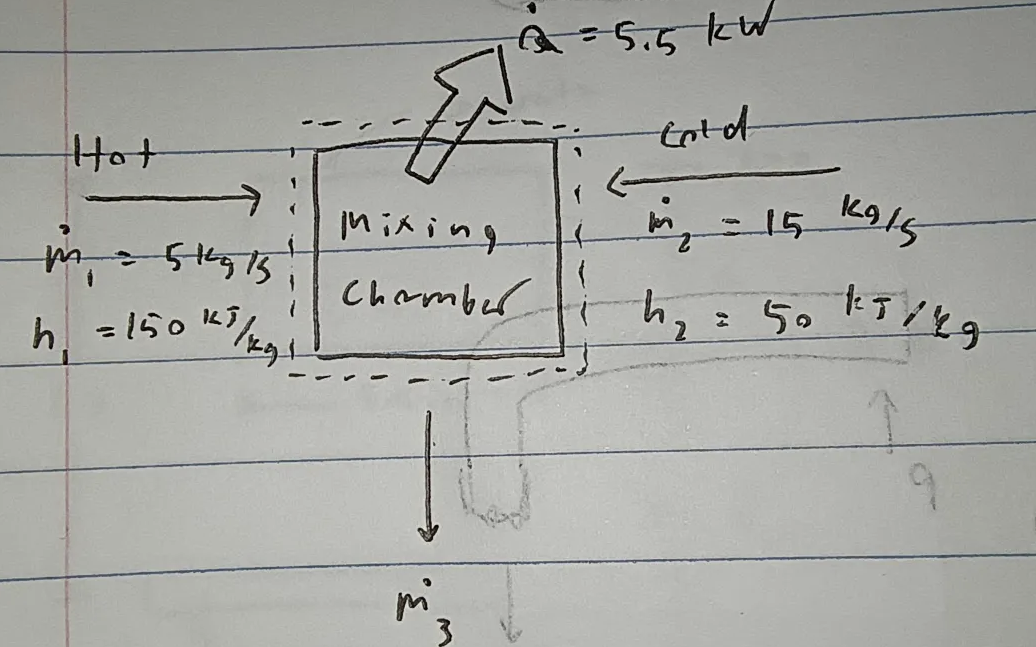
\includegraphics[width=0.6\textwidth]{5-73-1.png}
\end{center}
Writing the first law of thermodynamics for an open system:
\[\frac{dE}{dt} = \dot{Q}-\dot{W} +
\sum \dot{m_i}\left[h_i+\frac{1}{2}v_i^2+g z_i\right]
-\sum \dot{m_e}\left[h_e+\frac{1}{2}v_e^2+g z_e\right]\]
We can simplify the first law equation as follows:
\begin{itemize}
\item No work is done by the system ($\dot{W}=0$)
\item Steady state ($\frac{dE}{dt}=0$)
\item Neglect potential energy changes ($g z_i \approx g z_e$)
\item Neglect kinetic energy changes ($\frac{1}{2}v_i^2 \approx \frac{1}{2}v_e^2$)
\end{itemize}
Thus, the first law simplifies to:
\[0 = \dot{Q} + \left[\dot{m}_1 h_1 + \dot{m}_2 h_2\right] - \dot{m}_3 h_3\]
Substituting $\dot{m}_3 = \dot{m}_1 + \dot{m}_2$ and rewriting:
\[h_3 = \frac{\dot{Q} + \dot{m}_1 h_1 + \dot{m}_2h_2}{\dot{m}_1 + \dot{m}_2}\]
\underline{Note:} Since $\dot{Q}$ is heat transfer \textit{from the system} to the surroundings, it is a negative value by sign convention.
\[h_3 = \frac{[-5.5\,\text{kW}\cdot \frac{1\,\text{kJ/s}}{1\,\text{kW}}] + [5\,\text{kg/s}][150\,\text{kJ/kg}] + [15\,\text{kg/s}][50\,\text{kJ/kg}]}{[5 + 15\,\text{kg/s}]} = \boxed{74.725\,\text{kJ/kg}}\]

\section*{5-78E}
\vspace{-2em}
\begin{center}
    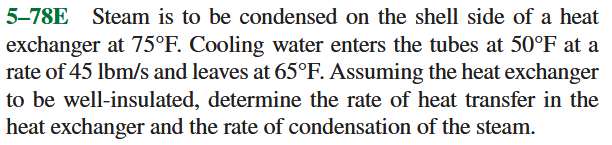
\includegraphics[width=0.7\textwidth]{5-78E.png}
\end{center}
Given:
\begin{itemize}
    \item State 1 (water entering the tube side)
    \begin{itemize}
        \item $\dot{m}_1 = 45$ lbm/s, $T_1 = 50^\circ$F
    \end{itemize}
    \item State 2 (water exiting the tube side)
    \begin{itemize}
        \item $T_2 = 65^\circ$F
    \end{itemize}
    \item State A (steam entering the shell side)
    \begin{itemize}
        \item Assuming that the steam is a saturated vapor
    \end{itemize}
    \item State B (condensed steam exiting the shell side)
    \begin{itemize}
        \item Assuming that the condensed steam is a saturated liquid
    \end{itemize}
    \item Condensation occurs in the shell side at $T = 75^\circ$F, so the temperatures at states A and B are both $75^\circ$F.\\\\
    From the saturated water tables at $T = 75^\circ$F, we can find $h_A = h_g = 1093.9$ Btu/lbm and $h_B = h_f = 43.07$ Btu/lbm.
\end{itemize}
\newpage\noindent
Find: 
\begin{itemize}
    \item Rate of heat transfer from the steam to the water, $\dot{Q}$ [Btu/s]
    \item Rate of condensation of the steam, or in other words, the mass flow rate of the condensed steam exiting $\dot{m}_B$ [lbm/s]
\end{itemize}
\begin{center}
    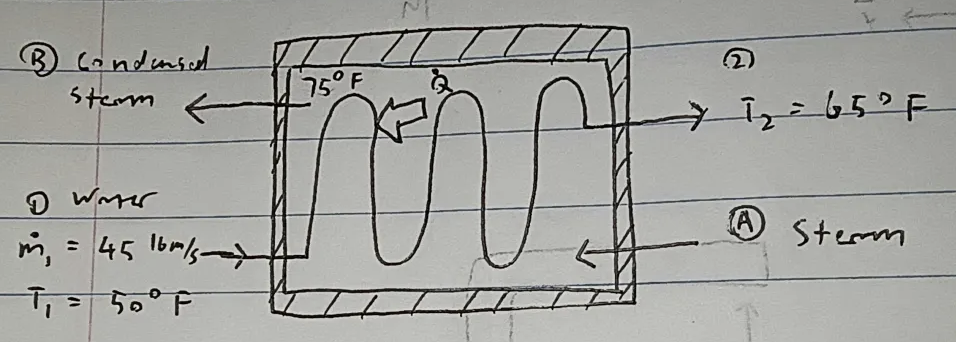
\includegraphics[width=0.6\textwidth]{5-78E-1.png}
\end{center}
\textbf{Control Volume: Tube}\\
Writing the first law of thermodynamics for an open system (tube side) to solve for the rate of heat transfer $\dot{Q}$:
\[\frac{dE}{dt} = \dot{Q}-\dot{W} +
\sum \dot{m_i}\left[h_i+\frac{1}{2}v_i^2+g z_i\right]
-\sum \dot{m_e}\left[h_e+\frac{1}{2}v_e^2+g z_e\right]\]
We can simplify the first law equation as follows:
\begin{itemize}
\item No work is done by the system ($\dot{W}=0$)
\item Steady state ($\frac{dE}{dt}=0$)
\item Neglect potential energy changes ($g z_i \approx g z_e$)
\item Neglect kinetic energy changes ($\frac{1}{2}v_i^2 \approx \frac{1}{2}v_e^2$)
\item By conservation of mass, $\dot{m}_1 = \dot{m}_2$
\end{itemize}
Thus, the first law simplifies to:
\[0 = \dot{Q} + \dot{m}_1 h_1 - \dot{m}_2 h_2\]
\[\dot{Q} = \dot{m}_1 (h_2 - h_1)\]
Like problem 5-28E, we can find the change in specific enthalpy either using the property tables (compressed liquid approximation) or using the specific heat at constant pressure ($c_p$). Note that while $c_p$ is constant for ideal gases, it is not constant for liquids. But we can still use it as an approximation since the water remains in the liquid phase and \textit{does not change phases}.\\\\
I will use the compressed liquid approximation method: the properties of the water is approx the same as the properties of a saturated liquid at the same temperature. From the saturated water tables, we can find $h_1 = h_f = 18.07$ Btu/lbm and $h_2 = h_f = 33.08$ Btu/lbm.
\[\dot{Q} = [45\,\text{lbm/s}][(33.08 - 18.07)\,\text{Btu/lbm}] = \boxed{675.45\,\text{Btu/s}}\]
\textbf{Control Volume: Shell}\\
The simplified first law equation for the shell side is the same as the tube side, except that the mass flow rates are $\dot{m}_A = \dot{m}_B$ and the specific enthalpies are $h_A$ and $h_B$:
\[0 = \dot{Q} + \dot{m}_A h_A - \dot{m}_B h_B\]
\[\dot{Q} = \dot{m}_B (h_B - h_A)\]
To find the rate of condensation of the steam, we can rearrange to solve for $\dot{m}_B$:
\[\dot{m}_B = \frac{\dot{Q}}{h_B - h_A} \]
We plug in the following values:
\begin{itemize}
    \item The rate of heat transfer $\dot{Q}$ found before is the same except now it is \textit{negative} because it is leaving the shell side
    \item Since we assumed that the steam is a saturated vapor at state A and a saturated liquid at state B, we can use the values of $h_A$ and $h_B$ found at $T=75^\circ$F from the saturated water tables. $h_A = h_g = 1093.9$ Btu/lbm and $h_B = h_f = 43.07$ Btu/lbm.
\end{itemize}
\[\dot{m}_B = \frac{[-675.45\,\text{Btu/s}]}{[43.07 - 1093.9\,\text{Btu/lbm}]} = \boxed{0.642\,\text{lbm/s}}\]

\section*{5-185}
\vspace{0em}
\begin{center}
    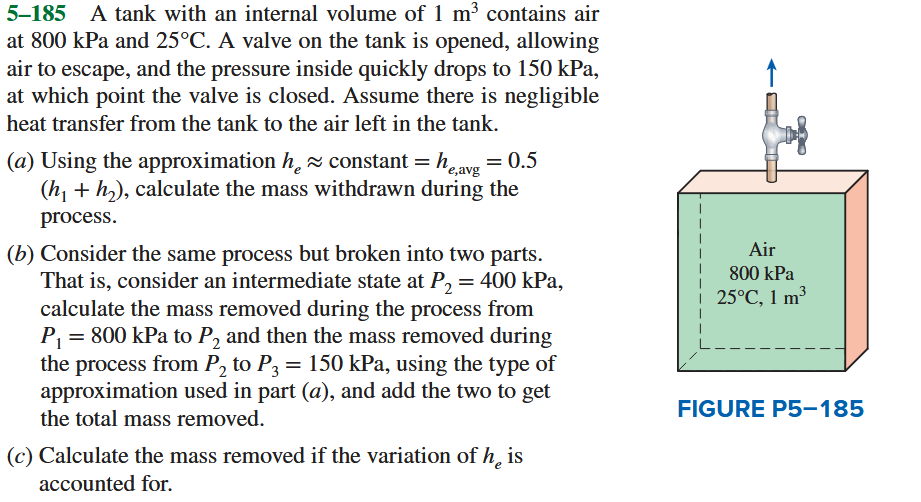
\includegraphics[width=1\textwidth]{5-185.png}
\end{center}
\newpage\noindent
Given:
\begin{itemize}
    \item State 1 (air in tank)
    \begin{itemize}
        \item $\vol_1 = 1\,\text{m}^3$, $P_1 = 800$ kPa, $T_1 = 25^\circ$C
    \end{itemize}
    \item State 2 (intermediate state in tank)
    \begin{itemize}
        \item $P_2 = 400$ kPa
    \end{itemize}
    \item State 3 (air in tank)
    \begin{itemize}
        \item $P_3 = 150$ kPa
    \end{itemize}
    \item State e (air exiting the system)
   \begin{itemize}
        \item Approximation $h_e \approx$ constant $=h_{e,\text{ avg}} = \frac{1}{2}(h_1 + h_3)$
    \end{itemize}
    \item No heat transfer ($\dot{Q}=0$) to the air
\end{itemize}
Find: 
\begin{itemize}
    \item The mass exiting the system $m_e$ [kg] using 3 different methods
\end{itemize}
Note that $h_e$ is the specific enthalpy of the air exiting the system, and $m_e$ is the total mass of the air that exits the system. Since the mass is changing over time, $\frac{dm}{dt} \neq 0$, so we cannot apply the steady state assumption.\\\\
\textbf{Method (a)}:\\
As always starting with the first law of thermodynamics for an open system:
\[\frac{dE}{dt} = \dot{Q}-\dot{W} +
\sum \dot{m_i}\left[h_i+\frac{1}{2}v_i^2+g z_i\right]
-\sum \dot{m_e}\left[h_e+\frac{1}{2}v_e^2+g z_e\right]\]
We can simplify the first law equation as follows:
\begin{itemize}
\item No work is done by the system ($\dot{W}=0$)
\item No heat transfer ($\dot{Q}=0$)
\item Neglect potential energy changes ($g z_i \approx g z_e$)
\item Neglect kinetic energy changes ($\frac{1}{2}v_i^2 \approx \frac{1}{2}v_e^2$)
\item $\dot{m}_i = 0$ because there is no inlet
\end{itemize}
Thus, the first law simplifies to:
\[\frac{dE}{dt} = -\dot{m}_e h_e\]
We can integrate both sides over time to find the total mass exiting the system:
\[E_3 - E_1 = -m_e h_e\]
The change in the \textit{total energy} of the system is equal to the change in the internal energy ($U$) of the air inside the tank since it is not flowing (so there is no flow work $h = u$).
\[E_3 - E_1 = m_3 u_3 - m_1 u_1\]
\underline{Note:} We only use enthalpy $h$ when there is flow work $P\svol$ (such as at the exit), but since there is no flow work at the inlet, we use internal energy $u$ instead of enthalpy $h$ for the states inside the tank.
\[\implies m_3 u_3 - m_1 u_1 = -m_e h_e\]
\[m_e = \frac{m_1 u_1 - m_3 u_3}{h_e}\]
Substituting in $h_e$:
\[m_e = 2\frac{m_1 u_1 - m_3 u_3}{(h_1 + h_3)}\]
To find the properties of the air at states 1 and 3, we can use the ideal gas properties of air table (A-17). But first we must find the temperature at state 3 using the i\textbf{sentropic relation}:
\[\boxed{\frac{T_3}{T_1} = \left(\frac{P_3}{P_1}\right)^{\frac{k-1}{k}}}\]
Where $k = c_p/c_{\svol}$ is the specific heat ratio.\\\\
We can assume that this is an isentropic process because there is no heat transfer and the process happens quick enough for there to be negligible frictional losses. Substituting in the values:
\[T_3 = T_1 \left(\frac{P_3}{P_1}\right)^{\frac{k-1}{k}} , \quad k = \frac{1.005}{0.718} = 1.399\]
\[T_3 = [298.15\,\text{K}] \left(\frac{[150\,\text{kPa}]}{[800\,\text{kPa}]}\right)^{\frac{1.399-1}{1.399}}=184.966\,\text{K}\]
Knowing the temperatures at states 1 and 3, we can use the specific heat constants to find the specific internal energies and specific enthalpies at states 1 and 3: 
\begin{itemize}
    \item State 1 (assuming $h=0$ and $u=0$ at $T=0$ K):
    \[u_1 = c_v (T_1 - 0) = 0.718 \times (298.15 - 0) = 214.07\,\text{kJ/kg}\]
    \[h_1 = c_p (T_1 - 0) = 1.005 \times (298.15 - 0) = 299.64\,\text{kJ/kg}\]
    \item State 3 (assuming $h=0$ and $u=0$ at $T=0$ K):
    \[u_3 = c_v (T_3 - 0) = 0.718 \times (184.966 - 0) = 132.80\,\text{kJ/kg}\]
    \[h_3 = c_p (T_3 - 0) = 1.005 \times (184.966 - 0) = 185.89\,\text{kJ/kg}\]
\end{itemize}
Also, we can find the mass of the air at states 1 and 3 using the ideal gas law:
\[m = \frac{P\vol}{RT}\]
\[m_1 = \frac{[800\times10^3\,\text{Pa}][1\,\text{m}^3]}{[287 \,\text{J/kg}\cdot\text{K}][298.15\,\text{K}]} = 9.349\,\text{kg}\]
\[m_3 = \frac{[150\times10^3\,\text{Pa}][1\,\text{m}^3]}{[287 \,\text{J/kg}\cdot\text{K}][184.966\,\text{K}]} = 2.825\,\text{kg}\]
Finally, we can substitute all the values into the equation for $m_e$:
\[m_e = 2\frac{[9.349\,\text{kg}][214.07\,\text{kJ/kg}] - [2.825\,\text{kg}][132.80\,\text{kJ/kg}]}{[299.64 + 185.89\,\text{kJ/kg}]} = \boxed{6.698\,\text{kg}}\]
\textbf{Method (b)}:\\
We do the same steps but with an intermediate state at state 2. We can find the temperature at state 2 using the isentropic relation:
\[T_2 = T_1 \left(\frac{P_2}{P_1}\right)^{\frac{k-1}{k}} = [298.15\,\text{K}] \left(\frac{[400\,\text{kPa}]}{[800\,\text{kPa}]}\right)^{\frac{1.399-1}{1.399}}= 244.66\,\text{K}\]
Then we can find the specific internal energy, specific enthalpy, and mass at state 2:
\[u_2 = c_v (T_2 - 0) = 0.718 \times (244.66 - 0) = 175.66\,\text{kJ/kg}\]
\[h_2 = c_p (T_2 - 0) = 1.005 \times (244.66 - 0) = 245.88\,\text{kJ/kg}\]
\[m_2 = \frac{[400\times10^3\,\text{Pa}][1\,\text{m}^3]}{[287 \,\text{J/kg}\cdot\text{K}][244.66\,\text{K}]} = 5.696\,\text{kg}\]
Then we can apply the first law of thermodynamics to the system between states 1 and 2, and then between states 2 and 3, to find the mass exiting the system $m_e$:
\[m_{e_{1\to2}} = 2 \frac{m_1u_1-m_2u_2}{h_1+h_2} = 2 \frac{[9.349\,\text{kg}][214.07\,\text{kJ/kg}] - [5.696\,\text{kg}][175.66\,\text{kJ/kg}]}{[299.64 + 245.88\,\text{kJ/kg}]} = 3.669\,\text{kg}\]
\[m_{e_{2\to3}} = 2 \frac{m_2u_2-m_3u_3}{h_2+h_3} = 2 \frac{[5.696\,\text{kg}][175.66\,\text{kJ/kg}] - [2.825\,\text{kg}][2.896\,\text{kJ/kg}]}{[245.88 + 185.89\,\text{kJ/kg}]} = 1.448\,\text{kg}\]
\[m_e = m_{e_{1\to2}} + m_{e_{2\to3}} = 3.669 + 2.896 = \boxed{6.565\,\text{kg}}\]
\textbf{Method (c):}\\
Now instead of treating $h_e$ as a constant, we treat it as a variable. Going back to the differential form of the first law:
\[\frac{dU}{dt} = -\dot{m}_eh_e\]
\[\frac{d}{dt}(m_\text{sys} u) = -\dot{m}_eh_e\]
\[\frac{d}{dt}(m_\text{sys} u) = m_\text{sys} \frac{du}{dt} + u \frac{dm_\text{sys}}{dt} = -\frac{dm_e}{dt}h_e\]
Note that by the conservation of mass, $\dot{m}_\text{sys} = -\dot{m}_e$, so we can rewrite:
\[\implies m_\text{sys} \frac{du}{dt} + u \frac{dm_\text{sys}}{dt} = \frac{dm_\text{sys}}{dt}h_e\]
Plug in for $u$ using the ideal gas relation $u = c_{\svol} T$ and $h = c_p T$:
\[m_\text{sys}c_{\svol} \frac{dT}{dt} + c_{\svol} T \frac{dm_\text{sys}}{dt} = \frac{dm_\text{sys}}{dt}c_p T\]
"Multiply through" by $dt$ and group differentials: 
\[m_\text{sys}c_{\svol}\,dT = (c_p-c_{\svol}) T\,dm_\text{sys}\]
\[\frac{dT}{T} = \left(\frac{c_p}{c_{\svol}} - 1\right)\frac{dm_\text{sys}}{m_\text{sys}}\]
Integrate both sides:
\[\int_{T_1}^{T_3} \frac{dT}{T} = \left(\frac{c_p}{c_{\svol}} - 1\right) \int_{m_{\text{sys},1}}^{m_{\text{sys},3}} \frac{dm_\text{sys}}{m_\text{sys}}\]
\[\ln\left(\frac{T_3}{T_1}\right) = \left(\frac{c_p}{c_{\svol}} - 1\right) \ln\left(\frac{m_{\text{sys},3}}{m_{\text{sys},1}}\right)\]
From before, we know that $m_{\text{sys},1} = 9.349$ kg from the ideal gas law. Plugging in the values to solve for $m_{\text{sys},3}$:
\[\ln\left(\frac{T_3}{T_1}\right)\left(\frac{c_p}{c_{\svol}} - 1\right)^{-1} =  \ln\left(\frac{m_{\text{sys},3}}{m_{\text{sys},1}}\right) = ln(m_{\text{sys},3}) - ln(m_{\text{sys},1})\]
\[ln(m_{\text{sys},3}) = ln(m_{\text{sys},1}) + \ln\left(\frac{T_3}{T_1}\right)\left(\frac{c_p}{c_{\svol}} - 1\right)^{-1}\]
\[m_{\text{sys},3} = m_{\text{sys},1} \cdot \exp\left[\ln\left(\frac{T_3}{T_1}\right)\left(\frac{c_p}{c_{\svol}} - 1\right)^{-1}\right]\]
\[m_{\text{sys},3} = 9.349 \cdot \exp\left[\ln\left(\frac{184.966}{298.15}\right)\left(\frac{1.005}{0.718} - 1\right)^{-1}\right] = 2.831\,\text{kg}\]
FINALLY,
\[m_e = m_{\text{sys},1} - m_{\text{sys},3} = 9.349 - 2.831 = \boxed{6.518\,\text{kg}}\]

\newpage

\section*{5-199}
\vspace{-2em}
\begin{center}
    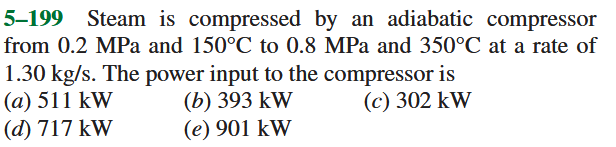
\includegraphics[width=0.7\textwidth]{5-199.png}
\end{center}
Given:
\begin{itemize}
    \item State 1 (entering compressor)
    \begin{itemize}
        \item $P_1 = 0.2$ MPa, $T_1 = 150^\circ$C
    \end{itemize}
    \item State 2 (exiting compressor)
    \begin{itemize}
        \item $P_2 = 0.8$ MPa, $T_2 = 350^\circ$C
    \end{itemize}
    \item $\dot{m}=\dot{m}_1 = \dot{m}_2= 1.3$ kg/s
    \item Adiabatic process (no heat transfer, $\dot{Q}=0$) with STEAM
\end{itemize}
Find: 
\begin{itemize}
    \item Power input to the compressor, $\dot{W}_\text{in}$ [kW]
\end{itemize}
Writing the first law of thermodynamics for an open system (compressor):
\[\frac{dE}{dt} = \dot{Q}-\dot{W} +
\sum \dot{m_i}\left[h_i+\frac{1}{2}v_i^2+g z_i\right]
-\sum \dot{m_e}\left[h_e+\frac{1}{2}v_e^2+g z_e\right]\]
We can simplify the first law equation as follows:
\begin{itemize}
\item No heat transfer ($\dot{Q}=0$)
\item Steady state ($\frac{dE}{dt}=0$)
\item Neglect potential energy changes ($g z_i \approx g z_e$)
\item Neglect kinetic energy changes ($\frac{1}{2}v_i^2 \approx \frac{1}{2}v_e^2$)
\end{itemize}
Thus, the first law simplifies to:
\[0 = -\dot{W} + \dot{m}_1 h_1 - \dot{m}_2 h_2 \implies \dot{W} = \dot{m}(h_1 - h_2)\]
Note that here $\dot{W}$ is the power done BY the system, so we substitute $\dot{W}_\text{in} = -\dot{W}$ to find the power input to the compressor:
\[\dot{W}_\text{in} = \dot{m}(h_2 - h_1)\]
Using the superheated water tables, we can find the specific enthalpies: $h_1 = 2769.1$ kJ/kg and $h_2 = 3162.2 $ kJ/kg.\\\\
Substituting into the first law equation:
\[\dot{W}_\text{in} = [1.3\,\text{kg/s}][3162.2 - 2769.1\,\text{kJ/kg}] = \boxed{511.03\,\text{kW},\, (a)}\]


\end{document}